\documentclass[12pt]{article}

\usepackage[utf8]{inputenc}
\usepackage{latexsym,amsfonts,amssymb,amsthm,amsmath}
\usepackage{graphicx}
\usepackage{hyperref}

\setlength{\parindent}{0in}
\setlength{\oddsidemargin}{0in}
\setlength{\textwidth}{6.5in}
\setlength{\textheight}{8.8in}
\setlength{\topmargin}{0in}
\setlength{\headheight}{18pt}



\title{Math 304 Take Home Exam}
\author{Colin Flanagan}

\begin{document}

\maketitle

\vspace{0.5in}
The rate of change of the mosquito population, $P$, (measured in millions of mosquitoes) in the area can be accurately modeled using the following Initial Value Problem:
\begin{align*}
    \frac{dP}{dt} &= kP(1-\frac{P}{M})-EP,\\
    \\
    P(0) &= P_0
\end{align*}
where $E$ is a constant that represents the effectiveness of insecticide spraying efforts, $M$ is
the local carrying capacity and is affected by efforts to reduce mosquito breeding
grounds, k is the population growth constant, $P_0$ is the initial population, and time $t$ is
measured in months. Current estimates suggest that there are approximately 10 million
mosquitoes living near the proposed site of the hospital. Data indicates that $P_0$ = 11 million
and $k$ = 1.2 for this mosquito population.\\

\subsection*{Task 1}
Use Desmos to investigate the effect of the parameter $E$ on solutions to the IVP. Recall that you can do this by graphing the right side of the differential equation and finding the
equilibrium solutions. Do they change in character as $E$ changes? Assume $0 \leq E \leq 1$. What happens to the mosquito population with different levels of insecticide spraying? Can spraying ever eliminate all mosquitoes? Write your answer in paragraph form and
include supporting graphs. \\
\\
Exponential growth model (Wrong):\\
\href{Desmos: }{https://www.desmos.com/calculator/t6skcegxqp}\\
\\
Parabola:\\
\href{Desmos: }{https://www.desmos.com/calculator/uokakj8edh}\\
After examining the desmos graph of the right side of the equation, one of the equilibrium solutions stays constant with changes in $E$, whilst the other is dependent on $E$. The first equilibrium solution is at 0,0 and the second equilibrium solution is found as a result of the quadratic equation for the right hand side of the model.

\vspace{1in} %Leave space for comments!


\subsection*{Exercise 2}
Use the information provided and Euler’s method to evaluate the following three mosquito population scenarios. $M = 10.5, E = 0.55; M = 6.0, E = 0.10; M = 9.0, E= 0.40$. To employ the Euler method on the right-hand side of this equation the following algorithm was followed
\begin{align*}
    P_{n+1} = P_n + h\space\cdot\space f(t,P)
\end{align*}
\raggedright
where $h$ is the step size/precision value, $P_n$ for the first step will be $P_0$, and $f(t,P)$ is our differential equation\\
\centering
     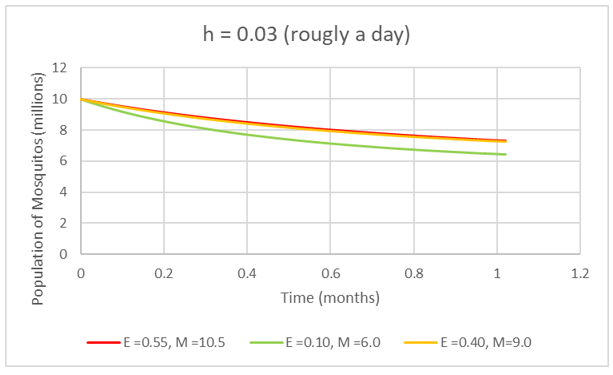
\includegraphics[width=0.8\linewidth]{Screenshot 2025-05-06 230916}\\
     Figure 1: Population of mosquitoes in millions over time in months solved using eulers method on the differential equation above with a step size of 0.03\\
\centering
     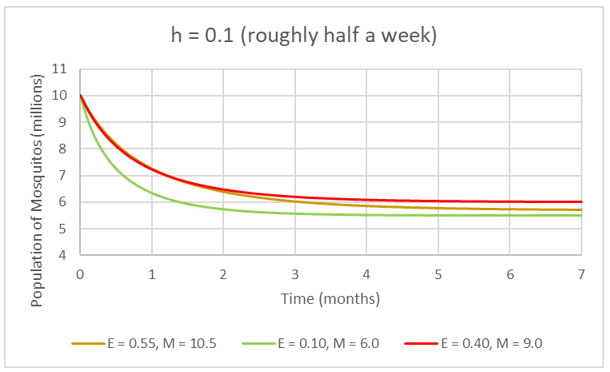
\includegraphics[width=0.8\linewidth]{Screenshot 2025-05-06 230922}\\
     Figure 2:Population of mosquitoes in millions over time in months solved using eulers method on the differential equation above with a step size of 0.1\\
\centering
     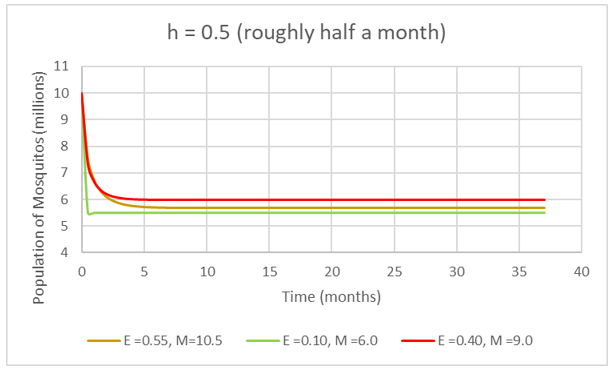
\includegraphics[width=0.8\linewidth]{Screenshot 2025-05-06 230928}\\
     Figure 3:Population of mosquitoes in millions over time in months solved using eulers method on the differential equation above with a step size of 0.5\\
\vspace{1in}
\raggedright
The colors of the functions indicate which one I would choose for a given length of time plan. Green functions are the ones I would choose and the red functions are ones I would not choose. These figures show a 1, 7, and 35 month plan using the different parameters. For all planning short term or long term we should choose the model where E = 0.10 and M = 6.0 so focusing efforts on destroying their breeding habitat and not on spraying. However, I would not advise total destruction especially if the mosquitoes are a keystone species, we should look at models of other local animals and how the mosquito population would effect them as well before making a major decision. In reality all of these models get the mosquito population in roughly the same place so in the short term dredging, but in the long term spraying is probably the best choice.
\end{document}